%%%%%%%%%%%%%%%%%%%%%%%%%%%%%%%%%%%%%%%%%%%%%%
\logvartrue
\chapter{Bacterial landlord: the microbiome concept}
%%%%%%%%%%%%%%%%%%%%%%%%%%%%%%%%%%%%%%%%%%%%%%
Bacteria have colonized thousands of different environments since the beginning of life on Earth. These environments include all the cavities and tissues, both inside and outside macroscopic organisms such as humans, plants and insects. The interaction between bacteria and their host is becoming more and more considered not only as a form of symbiosis but also as an evolution process that involves both host genome and all the different genomes of the bacterial communities associated with the host itself. The ecological community of commensal, symbiotic, and pathogenic microorganisms that thrive within a host is called ``microbiome''. In recent years, with the development of sequencing techniques able to obtain sequence of DNA directly from environmental sample, the analysis of microbiomes is becoming more and more affordable even by small laboratories. However, due to their great diversity, the comprehension of the bacterial dynamics involved in the host-microbial interaction remains far from our understanding. It is becoming more and more mandatory the development of approaches explicitly developed to cope with meta analyses regarding the host, the bacterial communities and the environment as a whole.\\
These topics have been explained in these papers:
\vspace{-5mm}
\begin{itemize}
\item Mengoni, A., Focardi, A., \textbf{Bacci, G.}, \& Ugolini, A. (2013). High genetic diversity and variability of bacterial communities associated with the sandhopper \textit{Talitrus saltator} (Montagu)(Crustacea, Amphipoda). \textit{Estuarine, Coastal and Shelf Science}, 131, 75-82.
\item \textbf{Bacci, G.}, Abdelrhman, K.F.A., Marras, B., Nistri, A., Schintu, M., Ugolini, A., \& Mengoni, A. The gut microbiota of talitrid amphipods provides insight into the ecology of supralittoral sediments detritivors. Manuscripts submitted to: \textit{FEMS Microbiology Ecology}.
\end{itemize}

\section{High genetic diversity and variability of bacterial communities associated with the sandhopper \textit{Talitrus saltator} (Montagu) (Crustacea, Amphipoda)}
Talitrid amphipods are one of the main components of the damp band of sandy beaches. They play important roles in the flow of energy and nutrients along the sandy beach ecosystem due to both their ability to feed on organic matter and providing nourishment for many species of beetles, fishes, birds and mammals. This work aimed to answer two key basic questions on the ecological interactions of dump band amphipods, using \textit{Talitrus saltator} as model species: $i)$ What is the composition, in taxonomic terms, of the bacterial community associated with single individuals and populations of \textit{T. saltator}? and $ii)$ is there individual or population-specific differentiation of the bacterial community?\\

\newpage
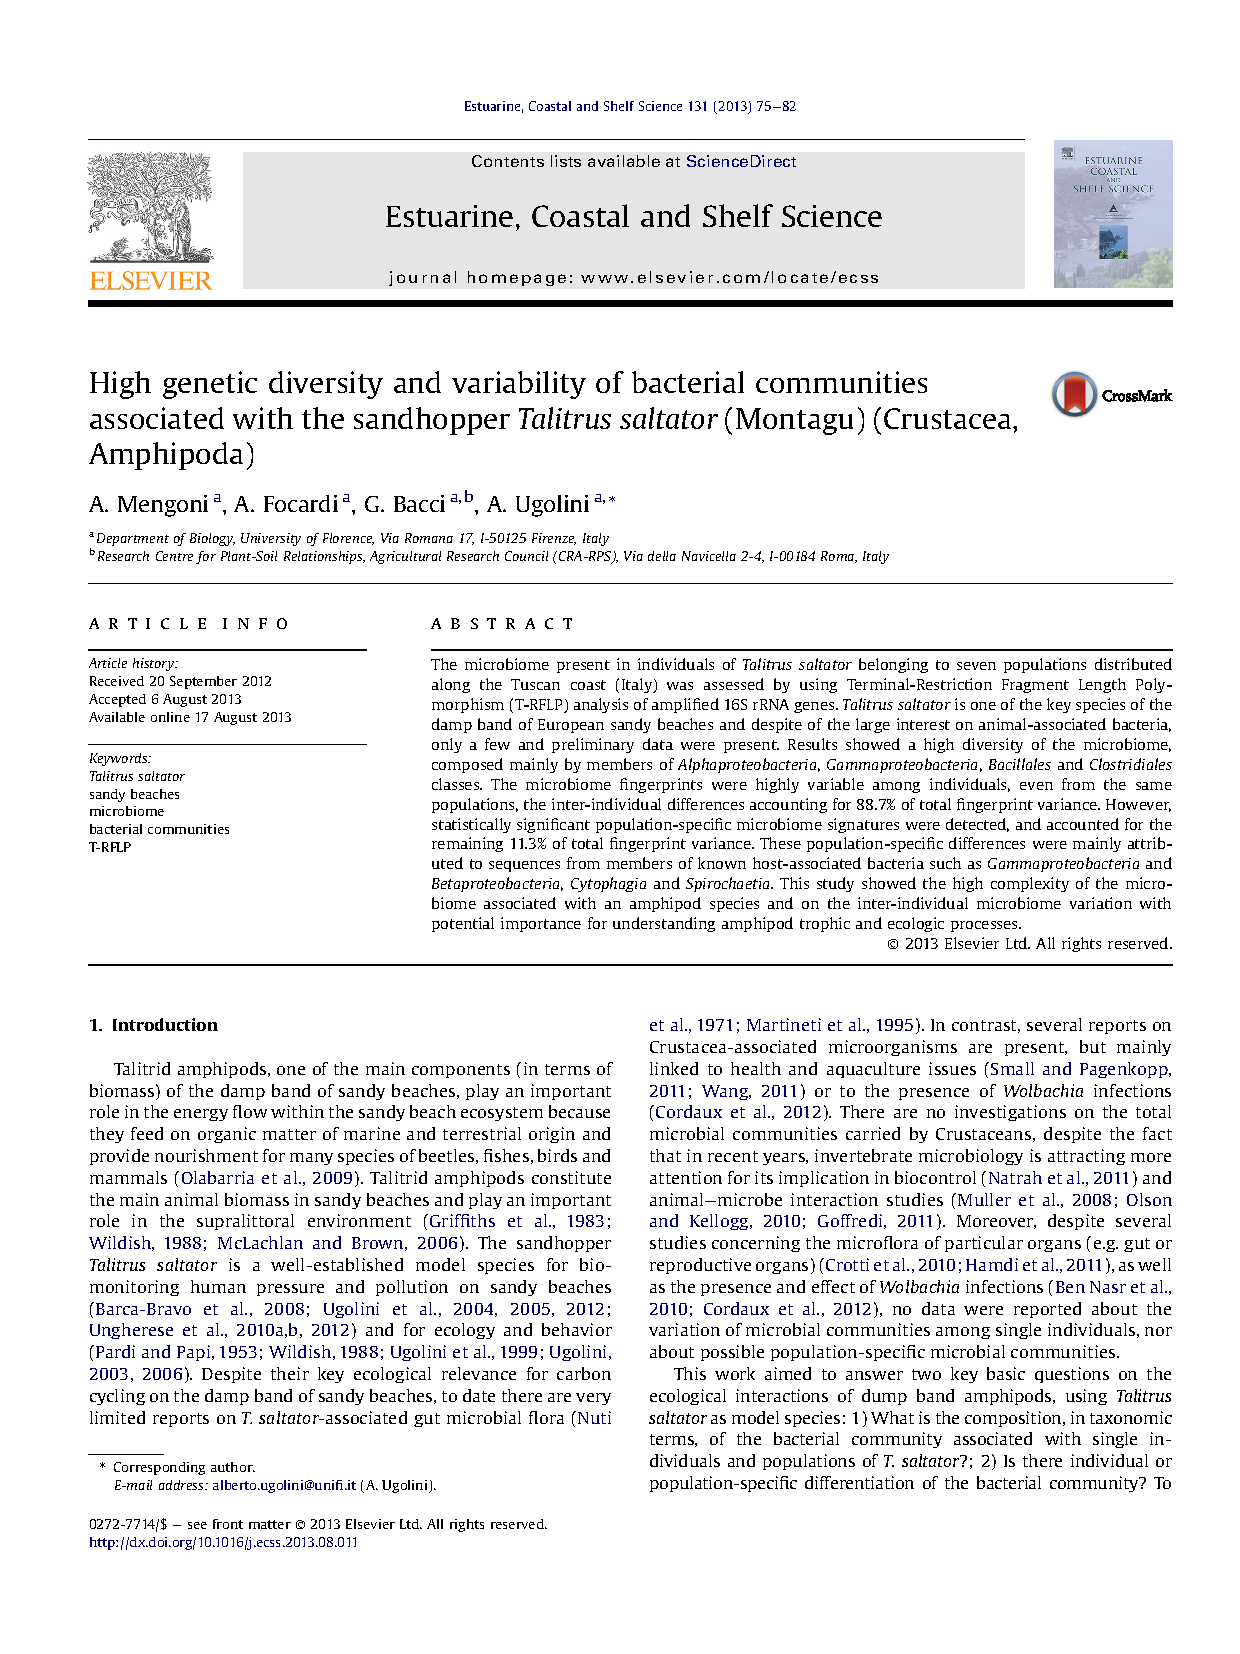
\includepdf[pages=-,offset=10mm 0, scale=0.9]{articles/talitri_1.pdf}
\newpage

%%%%%%%%%%%%%%%%%%%%%%%%%%%%%%%%%%%%%%%%%%%%%%%%%%%%%%%%%%%%%%%%%%%%%%%%%%%%%%%%%%%%%%%%%%%%%%%%%%%%%%%%%%%%%%%%%%%%%%%%%%%%%%%%%%%%%%%%%%%
%%%%%%%%%%%%%%%%%%%%%%%%%%%%%%%%%%%%%%%%%%%%%%%%%%%%%%%%%%%%%%%%%%%%%%%%%%%%%%%%%%%%%%%%%%%%%%%%%%%%%%%%%%%%%%%%%%%%%%%%%%%%%%%%%%%%%%%%%%%

\section{The gut microbiota of talitrid amphipods provides insight into the ecology of supralittoral sediments detritivors}
Talitrid amphipods sandhoppers and beach fleas are colonizers of the supralittoral zone and obtain most of their food from stranded materials, which include detrital marine angiosperms and macroalgae, as well as occasional death animals. Here, we report the characterization of gut microbiota of \textit{Talitrus saltator}, \textit{Talorchestia ugolinii}, \textit{Sardorchestia pelecaniformis}, \textit{Orchestia montagui}, collected in Sardinia (Italy). Microbiota were analyzed by metabarcoding analysis on amplified 16S rRNA V4 region and by quantification of family 48 glycosyl hydrolases genes, which are involved in cellulose degradation. Obtained results indicated the presence of a complex bacterial flora, including several members of \textit{Verrucomicrobia} in four out of the five species. Moreover, different gut microbiota taxonomic assemblages among the selected talitrid species were found. In particular, \textit{O. montagui} (which lives in close contact with \textit{Posidonia} banquette) gut microbiota was found to be the most different with respect to those of the other talitrids, being more abundant in members of \textit{Firmicutes}, \textit{Planctomycetes} and \textit{Actinobacteria}, and containing the highest level of family 48 glycosyl hydrolases genes. We conclude that talitrid amphipods harbour a complex gut microbiota which may be related to the habitat the different species colonizes.\\

\subsection{Introduction}
The microbiome, in particular the gut microbiome, is recognized as an ``extended genotype'' since it encodes a more versatile metabolome than the host \cite{sommer2013gut}. This is particularly relevant for animals which uses lignocellulosic compounds, as preferential food source (e.g. ruminants, termites). In the last years, a number of evidences are accumulating on the role of gut microbiota in determining or correlating with host's ecology in animals (see for instance \cite{becker2009first, basu2010association, bauer2000characterization, behar2008gut, dittmer2012influence}.\\
Talitrid amphipods sandhoppers and beach fleas are crustaceans living in the supralittoral zone and key components of the sandy beach food web \cite{calosi2005physiological, calosi2007physiological, morritt1988osmoregulation, morritt1989ionic, morritt1998physiological, ugolini1995distribution, pardi1986zonal}. Talitrid amphipods obtain most of their food from stranded materials, which include detrital marine angiosperms and macroalgae, as well as occasional death animals \cite{adin2003preferential}. However, among the Mediterranean talitrid taxa, species-specific habitat preferences have been observed. Indeed, some species (as \textit{Talitrus saltator}, \textit{Talorchestia ugolinii}, \textit{Sardorchestia pelecaniformis}) occur in the damp belt of sandy shores, while others (as \textit{Orchestia montagui}) are found under stranded algae and \textit{Posidonia} banquettes, independently from the type of substrate \cite{ugolini1995distribution, pavesi2013genetic}. Finally, for a third group of species (as \textit{Orchestia stephenseni}) the habitat seems to be more heterogeneous, the species being found in the damp of both sand sea shores and pools and lagoons backshore, as well as less within \textit{Posidonia} banquettes and also stranded detritus (e.g. see \cite{pavesi2013genetic, matthaeis2000isolation, lowry2013substrate, deidun2009considerations} and personal observations). Consequently, it is possible to hypothesize a differential food preference and, consequently ,a different taxonomic and functional pattern of gut microbiota among species. However, despite such intriguing question and the key ecological relevance for carbon cycling on the damp band of sandy beaches have talitrid amphipods \cite{griffiths1983kelp}, to date there are very limited reports on beach flea and sandhopper-associated microbial flora \cite{dittmer2012influence, mengoni2013high, nuti1971microrganisms}, and few studies have been performed in general on marine \textit{Crustacea} gut microbiota (e.g. see \cite{harris1993presence, zimmer2001hepatopancreatic, harris1993widespread}).\\
Aim of this work was the analysis of the composition and diversity of the gut microbiota from five different talitrid amphipods species (\textit{Talitrus saltator}, \textit{Talorchestia ugolinii}, \textit{Sardorchestia pelecaniformis}, \textit{Orchestia stephenseni}, \textit{Orchestia montagui}) which may be present in syntopy. In particular, the specific aim is to clarify the presence of gut microbiota signatures which may differentiate the five species, in relation to habitat and food preferences, then providing insight into their different ecology.

\subsection{Materials and Methods\label{par:kalmatmet}}

\subsubsection{Sampling}
Adults and sub-adults talitrids amphipods were collected in September 2013 from eight localities in Sardinia (Italy) (Table~\ref{tab:1kaltal}). For the locality of Giorgino beach, two different sampling points ca. 2 km aparts (named as Giorgino 1 and Giorgino 2) were selected and an additional sampling was also performed on September 2012 for Giorgino 1. In S. Giovanni di Sinis, two species were collected in syntopy (\textit{O. montagui} and \textit{O. stephenseni}). Immediately after collection, guts were excised from animals with sterile forceps and stored in DMSO/EDTA/NaCl preservative solution (20\% DMSO, 0.25 M disodium-EDTA, NaCl to saturation, pH 7.5) \cite{seutin1991preservation, dawson1998field}. Once arrived at the laboratory, samples were then stored at -80{\textdegree}C prior to DNA extraction. Pools composed by gut of ten animals per each species and locality were prepared. When available, for the same locality, two pools were prepared from animals collected at few distance (ca. 10 m), to take into account for possible population-based variation and substrate (e.g. sand and stranded material) heterogeneity. Twelve different pools were then prepared, accounting for a total of 120 single animals.\\
\begin{table}
\centering
\scriptsize
\begin{tabular}{c c c c c}
\hline
Code & Locality & Species & Longitude (E) & Latitude (N)\\
\hline\hline
KA11 & Centro 1{\textdegree} Sassu (Arborea) & {\itshape S. pelecaniformis} & 8{\textdegree}32'48.58{\textquotedbl} E & 39{\textdegree}48'7.08{\textquotedbl} N\\
KA9 & Centro 1{\textdegree} Sassu (Arborea) & {\itshape S. pelecaniformis} & 8{\textdegree}32'48.58{\textquotedbl} E &  39{\textdegree}48'7.08{\textquotedbl} N\\
KA2 & Giorgino 1 & {\itshape T. saltator} & 9{\textdegree}03'61.00{\textquotedbl} E & 39{\textdegree}11'11.41{\textquotedbl} N\\
KA4 & Giorgino 1 & {\itshape T. saltator} & 9{\textdegree}03'61.00{\textquotedbl} E & 39{\textdegree}11'11.41{\textquotedbl} N\\ 
KA5 & Giorgino 2 & {\itshape T. saltator} & 9{\textdegree}02'21.55{\textquotedbl} E & 39{\textdegree}10'26.31{\textquotedbl} N\\
KA12 & Is arenas & {\itshape T. ugolinii} & 8{\textdegree}28'46.35{\textquotedbl} E & 40{\textdegree} 4'13.00{\textquotedbl} N\\ 
KA13 & Is arenas & {\itshape T. ugolinii} & 8{\textdegree}28'46.35{\textquotedbl} E & 40{\textdegree} 4'13.00{\textquotedbl} N\\
KA8 & Maimoni (Cabras) & {\itshape O. montagui} & 8{\textdegree}24'02.36{\textquotedbl} E & 39{\textdegree}54'54.76{\textquotedbl} N\\
KA14 & Piscadeddus & {\itshape O. stephenseni} & 9{\textdegree}28'20.67{\textquotedbl} E & 39{\textdegree} 7'56.73{\textquotedbl} N\\
KA3 & S. Giovanni di Sinis (Cabras) & {\itshape O. montagui} & 8{\textdegree}26'11.03{\textquotedbl} E & 39{\textdegree}52'55.72{\textquotedbl} N\\
KA6 & S. Giovanni di Sinis (Cabras) & {\itshape O. stephenseni} & 8{\textdegree}26'51.42{\textquotedbl} E & 39{\textdegree}53'07.37{\textquotedbl} N\\
KA10 & Sa Rocca Tunda & {\itshape S. pelecaniformis} & 8{\textdegree}25'29.71{\textquotedbl} E &  40{\textdegree} 2'38.01{\textquotedbl} N\\
\hline
\end{tabular}
\caption{Sampled amphipod taxa and sampling locations. The locality with geographical coordinates of sampling point and sampled taxon is indicated.\label{tab:1kaltal}}
\end{table}

\subsubsection{DNA extraction, metabarcoding analysis and detection of cellulase genes}
DNA was extracted from gut tissues by using the QIAamp DNA Investigator Kit (Qiagen), quantified by agarose gel (0.8\% TAE w/v) electrophoresis and by spectrophotometric reading using the \href{http://www.tecan.com/2.2398/Infinite-200-NanoQuant-Specifications}{ Infinite{\textregistered} M200 PRO NanoQuant} (Tecan). From extracted DNA, the bacterial V4 region of 16S rRNA genes was amplified with V4 specific primers \cite{schriml201315th} and sequenced at the IGA Technology Services \href{http://www.igatechnology.com/}{http://www\-.igatech\-nology\-.com/}, Udine, Italy using an Illumina MiSeq apparatus with pair-end sequencing \cite{caporaso2012ultra}. Library preparation and demultiplexing have been performed following Illumina's standard pipeline. Sequence reads have been deposited under  the BioProject ID: PRJNA260027. Total bacterial titres were estimated by Real-Time PCR using a previously reported SybrGreen protocol \cite{bacci2014composition}. The same Real-Time PCR protocol (with annealing temperature decreased to 52{\textdegree}C) was used for detection and Real-Time quantification of glycosyl hydrolase family 48 (GHF48) genes by using GH48F/GH48R primer pair \cite{izquierdo2010diversity}. Standard curves for 16S rRNA and GHF48 have been prepared with serial dilutions of genomic DNA of \textit{Streptomyces coelicolor} A3 (2), which contains a putative GHF48 gene (SCO5456).\\

\subsubsection{Raw data processing}
Raw sequence data generated from Illumina sequencing were processed following several steps. First of all, sequences were quality trimmed with StreamingTrim 1.0 \cite{bacci2014streamingtrim}. Quality trimmed sequences were assembled and subjected to another quality control step with PANDAseq \cite{masella2012pandaseq}. Processed sequences were then subjected to the UPARSE pipeline \cite{edgar2013uparse}, in order to remove chimeric sequences (both in de novo and in reference mode) and to cluster them into Operational Taxonomic Units (OTUs). An identity threshold of 97\% has been used \cite{konstantinidis2007prokaryotic}. Representative sequences obtained from the UPARSE clustering were taxonomically classified using the SINA standalone classifier using the ``Ref NR 99'' as reference database \cite{pruesse2012sina}. After taxonomic classification we removed from our dataset all OTUs not assigned at least at Bacteria domain.\\

\subsubsection{Biodiversity indexes analysis and statistical analysis}
Rarefaction curves have been generated using the OTU assignments. Sample assignments have then be rarefied using a number of random subsamples equal to the number of assignments of the smaller sample Shannon, Richness and Evenness indexes were calculated on the rarefied samples; In order to investigate the presence of species-specific patterns in the metabarcoding data of gut microbiota of the talitrid amphipds OTU abundances were then used to perform a Canonical Correlation Analysis. Real-Time PCR data were statistically analyzed by one- ay ANOVA. All statistical analyses were performed with the R software with the following packages: vegan \cite{dixon2003vegan, oksanen2007vegan}; igraph \cite{csardi2006igraph} and ggplot2 \cite{ginestet2011ggplot2}.\\

\subsubsection{Network construction and clustering}
In order to generate a OTUs network displaying patterns of correlation between each OTU, we calculated Spearman's correlations between all OTUs in our dataset, regardless of the sample of origin. Each OTU has been considered as a vertex inside the network and an edge between two OTUs has been created only if the Spearman's correlation coefficient between those OTUs was statistically significant (p {\textless} 0.05) and r {\textgreater} 0.5. In this way we generate an edge linking two OTUs only when there is a statistically significant and high degree of correlation between the two OTUs. In order to inspect the OTU distribution in the generated network the Markov Cluster Algorithm (MCL) was used \cite{van2000graph}. This method uses only one parameter in order to choose the number of cluster to generate; this parameter is called ``inflation values'' and it can range between 1.2 and 5.0 as reported by the author of the algorithm. In order to find the ``inflation value'' (IF) resulting in an informative number of clusters we used the ``intracluster clustering coefficient'' (ICCC) method \cite{lima2008reticulate}). Thus, we generated 39 different clusters using all IF values between 1.2 and 5.0 increasing the IF value by 0.1 each time and calculating the ICCC value for each clustering. Finally, the IF value that maximize the ICCC was 1.4 with the generation of 5 clusters. A representation of the generated network was drawn using Gephi \cite{bastian2009gephi} with the ``Force Field layout''; nodes were colored based on the cluster attribution.\\

\subsection{Results and Discussion}

\subsubsection{Representativeness and diversity of gut microbiota}
The metabarcoding analysis of 16S rRNA genes from the twelve gut DNA samples, representing five different talitrid species resulted in a relatively good coverage of bacterial diversity, with almost all samples reaching saturation or near saturation values (Figure~\ref{fig:1talkal}). A total number of 7606010 (15212020 paired-end) reads was obtained with 410864 to 846775 reads per sample. After clustering at 97\% identity a total of 1004 OTUs were identified in the twelve samples (Table SM1).\\
\begin{figure}[!tb]
	\centering
	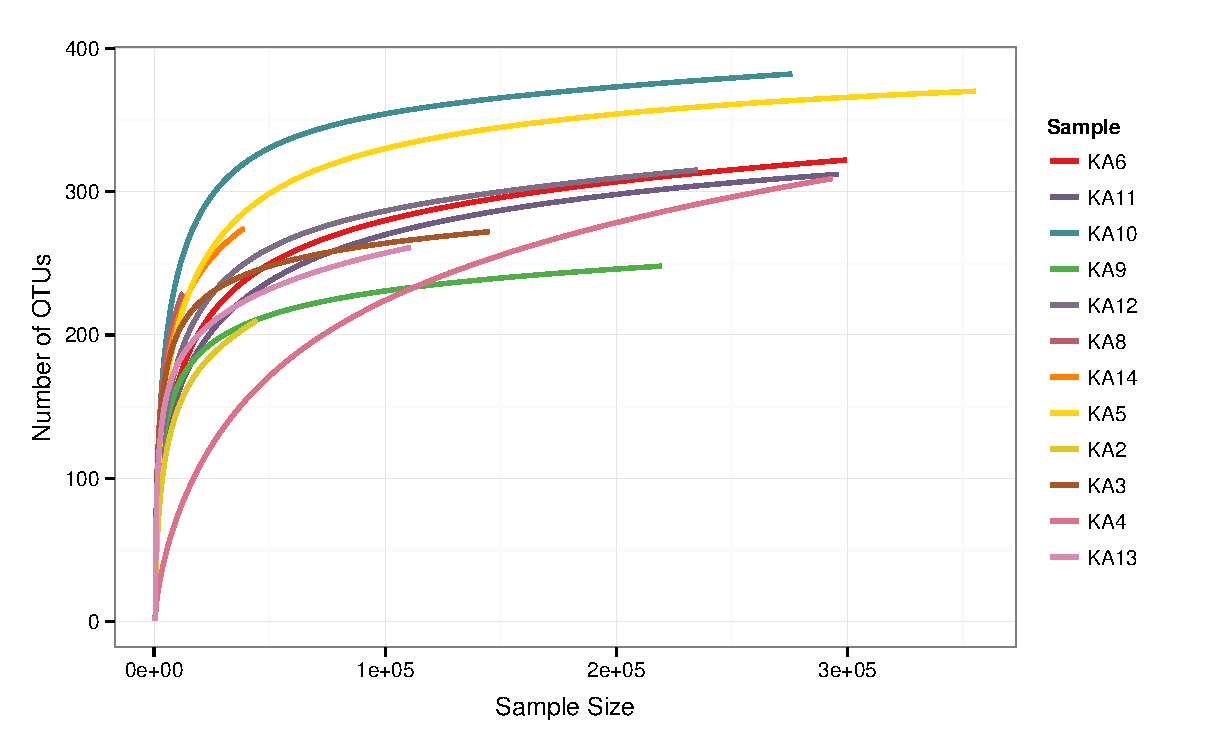
\includegraphics[width=1\textwidth]{./figures/Chapter_6/Figure_1_talkaled.eps}
  	\caption{Representativeness of sampled gut microbiota. The number of Operating Taxonomic Units (OTUs) as a function of
the number of sampled sequences is reported. The sequences were sampled with a step size of 100 sequences in order to
generate smooth curves. The asymptotic trends of curves indicate that a reasonable number of reads has been generated
in order to inspect the diversity of each sample. The different end values indicates variable numbers of clustered
sequences per sample.\label{fig:1talkal}}
\end{figure}
The analysis of community diversity for each samples (Table~\ref{tab:2kaltal}) showed  the lowest values for all three indices (Richness, Shannon and Evenness) for KA6 sample (\textit{O. montagui}), while the highest values were reached by the other \textit{O. montagui} sample (KA3), for Shannon and Evenness and by \textit{S. pelecaniformis} (KA10) for Richness. However, no statistically significant differences were found in relation to both talitrid species and locality of sampling (Table SM2).\\
\begin{table}
\centering
\scriptsize
\begin{tabular}{ c c c c c c }
\hline
Species & Locality & code & Richness & Shannon H & Evenness\\
\hline\hline
{\itshape O. montagui} & S. Giovanni di Sinis (Cabras) & KA3 & 322 & 3.995 & 0.692\\
{\itshape O. montagui} & Maimoni (Cabras) & KA8 & 229 & 0.497 & 0.091\\
{\itshape O. stephenseni} & Piscadeddus & KA14 & 274 & 0.931 & 0.166\\
{\itshape O. stephenseni} & S. Giovanni di Sinis (Cabras) & KA6 & 366 & 2.846 & 0.482\\
{\itshape S. pelecaniformis} & Centro 1{\textdegree} Sassu (Arborea) & KA11 & 294 & 3.473 & 0.611\\
{\itshape S. pelecaniformis} & Centro 1{\textdegree} Sassu (Arborea) & KA9 & 338 & 2.207 & 0.379\\
{\itshape S. pelecaniformis} & Sa Rocca Tunda & KA10 & 430 & 3.957 & 0.653\\
{\itshape T. saltator} & Giorgino & KA2 & 413 & 3.485 & 0.579\\
{\itshape T. saltator} & Giorgino & KA4 & 205 & 0.783 & 0.147\\
{\itshape T. saltator} & Giorgino & KA5 & 311 & 1.790 & 0.312\\
{\itshape T. ugolinii} & Is arenas & KA & 372 & 3.120 & 0.527\\
{\itshape T. ugolinii} & Is arenas & KA12 & 287 & 2.564 & 0.453\\
\hline
\end{tabular}
\caption{Diversity indices of microbiota. Diversity indices of gut microbiota in the twelve metabarcoding samples.\label{tab:2kaltal}}
\end{table}

\subsubsection{Species-specific signatures of gut microbiota}
Numerous evidences indicate that animals co-evolve with their gut microbiota \cite{ley2008worlds}. Consequently, species-specific patterns in the metabarcoding data of gut microbiota of the talitrids amphipds were inspected. Figure~\ref{fig:2talkal} reports the CCA  results, which indicate the presence of clearly separate clusters for the five species under analysis (\textit{O. montagui}, \textit{S. pelecaniformis}, \textit{T. saltator}, \textit{T. ugolinii}, \textit{O. stephensenii}), then supporting the hypothesis that amphipod digestive tracts host species-specific bacterial communities, which may be related to both the phylogeny and to potential dietary differences among the amphipod species, as exemplified in vertebrates \cite{ley2008worlds}.\\
\begin{figure}[!tb]
	\centering
	\includegraphics[width=0.7\textwidth]{./figures/Chapter_6/Figure_2_talkaled.eps}
  	\caption{Species-specific signatures of gut microbial community composition. Canonical Correlation Analysis (CCA) based
on OTU assignments to the bacterial taxonomy.\label{fig:2talkal}}
\end{figure}
As recently proposed for soil bacterial communities \cite{barberan2011using}, network analysis of significant taxon co-occurrence patterns could be useful to decipher the structure of complex microbial communities. Several works have shown recently that network analysis of co-occurrence may allow to define community patterns in several environments (for examples \cite{berry2014deciphering, boutin2014inter, williams2014demonstrating, geng2014co} see). Consequently, to further inspect the species-specific signatures of our amphipod gut microbiota a network analysis was conducted on Pearson's correlations among OTUs. This analysis, coupled with a k-means clustering, highlighted the presence of five taxonomically differentiated groups (clusters) of co-occurring OTUs (Figure~\ref{fig:3talkal}), in particular concerning \textit{Proteobacteria}, \textit{Actinobacteria} and \textit{Firmicutes}. Such clusters showed different representation in the five amphipod taxa (Figure SM1). In particular, cluster 4 was practically absent in \textit{S. pelecaniformis}, while the other clusters showed both a high variability among species, as well as among samples within the same species.\\
\begin{figure}[!tb]
	\centering
	\includegraphics[width=0.9\textwidth]{./figures/Chapter_6/Figure_3_talkaled.eps}
  	\caption{Network-based signatures of species-specific microbiota composition. Correlation network of OTU assignments. Each connection stands for a high degree of correlation between the two OTUs connected (Spearman's correlation r {\textgreater} 0.6 and p-value {\textless} 0.05). The size of each node in the network is proportional to its degree (number of connection of the node). The color of each node corresponds to a cluster obtained with the MCL algorithm with an ``inflation value'' equal to 1.4 (see section~\ref{par:kalmatmet}). Clusters have been defined after a k-means clustering.\label{fig:3talkal}}
\end{figure}

\subsubsection{Taxonomic differences in gut microbiota among talitrid species}
To evaluate which bacterial taxa mostly contribute to the interspecific differences of gut microbiota, OTUs were then assigned to bacterial phylogeny (Table SM3). Figure~\ref{fig:4talkal} shows the overall representation of taxonomic composition of gut microbiota, which highlight similar patterns, among all samples, with differences both within the same species, and among species. In particular, it could be worth of mentioning that \textit{Verrucomicrobia} were present in four out of five species (absent from all \textit{S. pelecaniformis} samples), as well as the group \textit{Deinococcus/Thermus} absent in both \textit{Orchestia} species. \textit{Verrucomicrobia} are particularly intriguing since this phylum, closely related to \textit{Planctomycetes} and \textit{Chlamydiae}, is considered to be particularly frequent in nonhost-assocaited environments, as soil and waters \cite{buckley2001environmental,freitas2012global}. \textit{Verrucomicrobia} have been suspected to contribute to energy generation from fermentable substrates in the human gut \cite{arumugam2011enterotypes} and \textit{Verrucomicrobia} have been found as particularly abundant after antibiotic treatment \cite{dubourg2013high}. We cannot consequently exclude that \textit{Verrucomicrobia} (present in all but \textit{S. pelecaniformis} samples) may have a role in some hypothetical differential nutrient assimilation in those talitrid species and in differential resilience toward environmental disturbance, which is frequent in sandy beaches \cite{defeo2009threats, ugolini2012sandhoppers, ugolini2005heavy, ugolini2008amphipod, ungherese2010relationship, moffett1998impact}.\\
\begin{figure}[!tb]
	\centering
	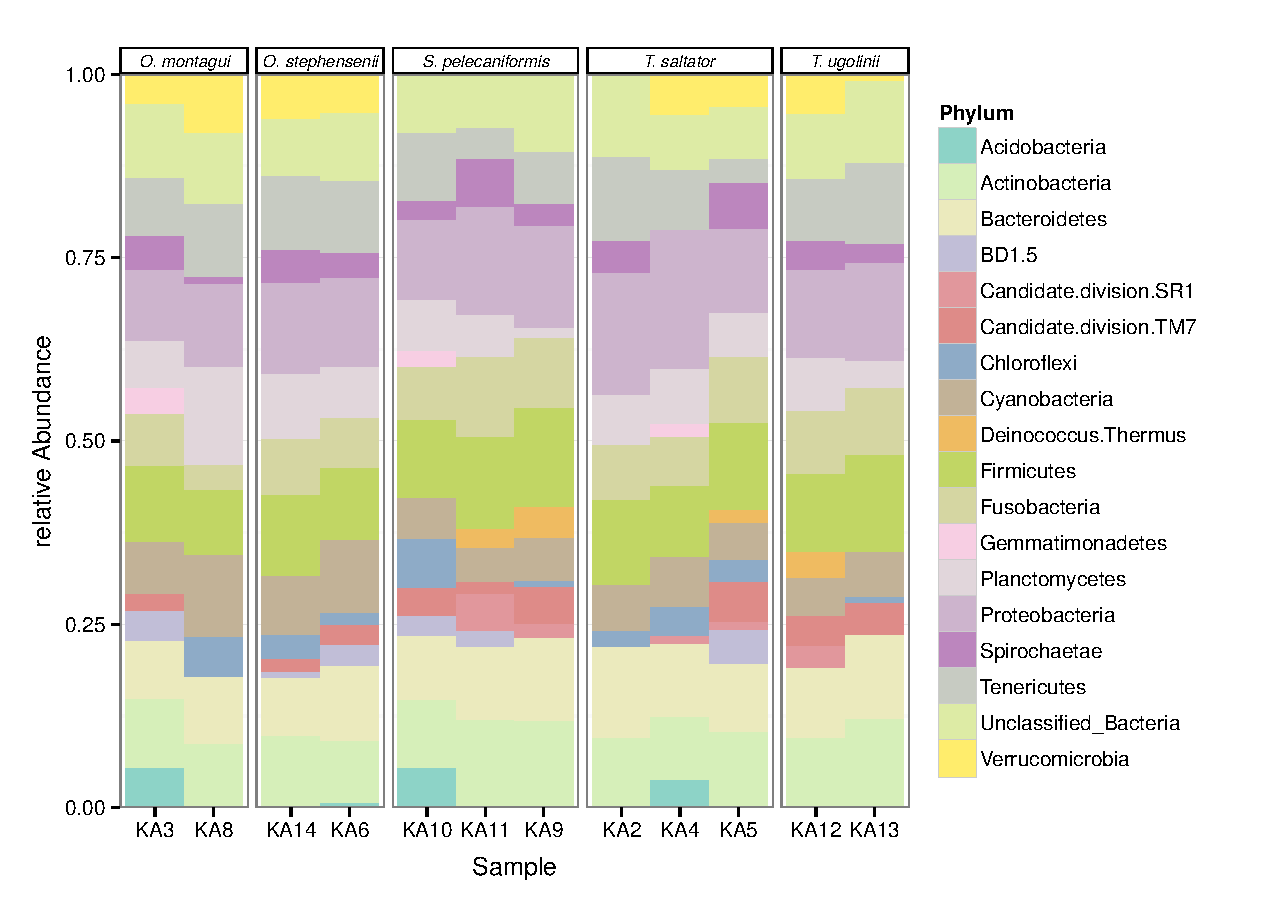
\includegraphics[width=1\textwidth]{./figures/Chapter_6/Figure_4_talkaled.eps}
  	\caption{Taxonomic composition of gut microbiota. Relative abundances barplot showing the relative abundance of bacterial phyla in each gut sample.\label{fig:4talkal}}
\end{figure}
To more in deep clarify the relative contribution of each phylum in species-specific gut microbiota signatures, a similarity percentage (simper) analysis was conducted (Table~\ref{tab:3kaltal}, Table SM3). In general, the phyla mostly contributing to differences between talitrid species are the most abundant, as \textit{Proteobacteria} (5.5\%-9.1\%), \textit{Firmicutes }(5.2\%-9.0\%), \textit{Bacteriodetes} (5.0\%-6.3\%), and \textit{Actinobacteria} (4.9\%-8.6\%). Interestingly, \textit{O. montagui}, which inhabits within the Posidonia banquettes  and macroalgae mat, shows the highest percentage of variance for \textit{Planctomycetes} in all pairwise comparisons, as well as among the highest percentage of variance for \textit{Firmicutes} also. \textit{Planctomycetes} have been found to densely populate the alkaline part of the hindgut of soil-feeding termites (\textit{Cubitermes} spp.) \cite{kohler2008novel} and to strongly vary with diet in humans \cite{cayrou2013molecular}. Moreover, \textit{Planctomycetes} constitute a large part of bacterial biofilms found on macroalgae \cite{lage2014planctomycetes}. The relative importance of \textit{Firmicutes} and \textit{Planctomycetes} in differentiating \textit{O. montagui }gut\textit{ }microbiota from those of the other talitrid species, may be due to the habitat of this species, possibly linked to the potential higher cellulose content of its diet. Of course confirmatory experiments under controlled conditions are needed to better evaluate the relative contribution of diet with respect to species in determining the specific of \textit{O. montagui }gut microbiota, especially in comparison with \textit{O. stephenseni}, which has been found in syntopy in the S. Giovanni di Sinis site (KA3 and KA6, Table~\ref{tab:1kaltal}).\\
\begin{landscape}
\begin{table}
\centering
\tiny
\begin{tabular}{ p{0.04\textwidth} p{0.04\textwidth} p{0.04\textwidth} p{0.04\textwidth} p{0.04\textwidth} p{0.04\textwidth} p{0.04\textwidth} p{0.04\textwidth} p{0.04\textwidth} p{0.04\textwidth} p{0.04\textwidth} p{0.04\textwidth} p{0.04\textwidth} p{0.04\textwidth} p{0.04\textwidth} p{0.04\textwidth} p{0.04\textwidth} p{0.04\textwidth} p{0.04\textwidth}}
\hline
 & Acido\-bacte\-ria & Actino\-bacte\-ria & Bacte\-roide\-tes & BD1.5 & SR1 & TM7 & Chlo\-rofl\-exi & Cyano\-bacte\-ria & Denico\-ccus/Ther\-mus & Fir\-micu\-tes & Fuso\-bacte\-ria & Placto\-myce\-tes & Proteo\-bacte\-ria & Spir\-ocha\-ete & Tene\-ricu\-tes & Unclas\-si\-fied & Verruco\-micro\-bia & Gemmati\-monade\-tes\\
\hline\hline
Os vs Sp & 0.65\% & 5.94\% & 5.54\% & 0.11\% & 0.11\% & 0.11\% & 0.66\% & 0.64\% & 0.11\% & 5.86\% & 0.36\% & 2.41\% & 7.81\% & 0.20\% & 0.34\% & 0.33\% & 0.53\% & NA\\
Os vs Tu & NA & 5.58\% & 4.99\% & 0.13\% & NA & 0.13\% & 0.13\% & 0.89\% & 0.12\% & 5.23\% & 0.54\% & 2.70\% & 6.82\% & 0.16\% & 0.40\% & 0.40\% & 0.69\% & NA\\
Os vs Om & 0.36\% & 6.50\% & 5.75\% & 0.17\% & NA & NA & NA & 1.16\% & NA & 8.68\% & 0.70\% & 6.10\% & 7.03\% & 0.21\% & 0.31\% & 0.51\% & 0.70\% & NA\\
Os vs Ts &NA & 7.73\% & 5.69\% & 0.15\% & NA & 0.15\% & 0.30\% & 0.59\% & NA & 7.02\% & 0.74\% & 2.80\% & 9.09\% & 0.26\% & 0.43\% & 0.42\% & 0.65\% & NA\\
Sp vs Tu & 0.67\% & 4.88\% & 5.07\% & 0.10\% & 0.10\% & NA & 0.70\% & 0.77\% & 0.09\% & 5.45\% & 0.32\% & 1.75\% & 6.20\% & 0.29\% & 0.17\% & 0.35\% & 0.23\% & NA\\
Sp vs Om & 0.57\% & 7.23\% & 6.34\% & 0.16\% & 0.16\% & 0.15\% & 0.31\% & 1.06\% & 0.15\% & 9.02\% & 1.00\% & 5.14\% & 6.94\% & 0.35\% & 0.35\% & 0.43\% & 0.34\% & 0.12\%\\
Sp vs Ts & 0.27\% & 8.24\% & 5.94\% & 0.15\% & 0.15\% & 0.14\% & 0.86\% & 0.56\% & 0.14\% & 8.23\% & 0.80\% & 1.25\% & 8.07\% & 0.45\% & 0.29\% & 0.44\% & 0.07\% & NA\\
Tu vs Om & 0.29\% & 7.88\% & 5.78\% & 0.17\% & NA & 0.17\% & NA & 1.14\% & NA & 8.89\% & 0.95\% & 5.66\% & 5.73\% & 0.10\% & 0.31\% & 0.51\% & 0.40\% & NA\\
Tu vs Ts & NA & 8.58\% & 5.88\% & NA & NA & 0.15\% & 0.15\% & 0.76\% & 0.15\% & 8.23\% & 0.84\% & 1.61\% & 7.21\% & 0.17\% & 0.34\% & 0.50\% & 0.25\% & NA\\
Om vs Ts & 0.65\% & 7.16\% & 5.98\% & 0.18\% & NA & 0.18\% & 0.52\% & 0.86\% & NA & 9.03\% & 0.87\% & 6.23\% & 7.63\% & 0.31\% & 0.41\% & 0.51\% & 0.59\% & 0.14\%\\
\hline
\end{tabular}
\caption{Species-specificity of bacterial phyla. Results of simper analysis. The percentage of variance attributed to each phylum in pairwise comparisons of talitrid species is reported. In bold pairwise comparison with \textit{O. montagui}. Om,, \textit{O. montagui}; Sp, \textit{S. pelecaniformis}; Ts, \textit{T. saltator}; Tu, \textit{T. ugolinii}; Os, \textit{O. stephenseni}.\label{tab:3kaltal}}
\end{table}
\end{landscape}

\subsubsection{Cellulolytic bacteria may contribute to \textit{O. montagui} gut microbiota difference}
From the analysis of taxonomic pairwise differences in gut microbiota (Table~\ref{tab:3kaltal}), it emerged that among the most important bacterial phyla, those of \textit{Firmicutes} and \textit{Planctomycetes} were particularly related to possible dietary/habitat differences between \textit{O. montagui} and the other talitrids. Both \textit{Firmicutes} and \textit{Planctomycetes} includes cellulose-degrading strains \cite{kulichevskaya2007schlesneria, schwarz2001cellulosome}. Additionally, a large proportion of \textit{Actinobacteria}(Figure~\ref{fig:4talkal}), which are well known to include many cellulolytic strains \cite{ljungdahl1985ecology}, has been found in all talitrid species. These evidence raised the question if the proportion of cellulosolytic bacteria with respect to the total bacterial load of the gut, may indeed be different between amphipod talitrids. However, from the molecular point of view, it is difficult to have a global overview of all genes encoding cellulases in a sample. Cellulase systems are in fact complex assemblages of multifunctional glycosyl hydrolases \cite{schwarz2001cellulosome}. Many families of glycosyl hydrolases have been found \cite{lynd2002microbial}, hampering the possibility to develop universal primers for PCR detection of all known cellulases. However, family 48 glycosyl hydrolases are well represented in many model cellulolytic clostridia and actinobacteria \cite{lynd2002microbial, beloqui2010diversity}.Primer pairs have been developed for 48 glycosyl hydrolases genes identification and quantification in environmental samples \cite{izquierdo2010diversity,pereyra2010detection}, in particular for clostridia and actinobacteria \cite{izquierdo2010diversity}. Since in our study a considerable fraction of recovered taxa fall within both \textit{Firmicutes} and \textit{Actinobacteria} (approx. 25\% of reads) we decided to investigate the presence of family 48 glycosyl hydrolases genes in amphipod gut microbiota. Results of the qPCR analysis are reported in Table 4. Interestingly, \textit{O. montagui} gut samples contained a higher ratio of GHF48 genes/16S rRNA genes (considered as estimators of the total number of bacterial cells) with respect to the other talitrid species, suggesting that indeed the different microbiota present in \textit{O. montagui} gut may be partly related to a higher prevalence of feeding on cellulose-rich substrates by this species.\\

\subsection{Conclusions}
Talitrid amphipods inhabiting supralittoral environment obtain most of their food from stranded materials, which include debris of various origin, as death animal organisms, macroalgae and plants (as land plants and \textit{P. oceanica} in the Mediterranean sea) \cite{adin2003preferential, colombini2011food}. In particular, due to the presence of low digestible components including lignocellulosic compounds in macroalgae and plants, we can hypothesize that a cellulosolytic bacterial flora in the digestive tract of talitrids could contribute in cellulose degradation. Indeed, previous authors \cite{nuti1971microrganisms, olabarria2009intraspecific} reported the presence of cellulose-degrading bacterial strain in the gut of talitrid amphipods, supporting the hypothesis of the involvement of gut microbiota in carbon source assimilation by such species. Here, we indicate that among the sampled species, which colonizes different microhabitats, \textit{O. montagui} (which is found within \textit{Posidonia} and macroalgae banquettes) harbors a different gut microbiota with respect to the other species. The \textit{O. montagui} gut microbiota includes more taxa known to be involved in cellulose degradation and an analysis of family 48 glycosyl hydrolases (one of the cellulase genes) indicated that indeed \textit{O. montagui} gut harbor a higher number of cellulose-degrading cells than the other talitrids. We conclude that the different ecological behavior of \textit{O. montagui} (a colonizer of \textit{Posidonia} banquettes) could be related also to a different taxonomic and functional composition of its gut microbiota. We cannot however, a priori exclude that a contribution of host encoded glycosyl hydrolases to food digestion could be present in \textit{O. montagui} and in the other talitrid amphipods, as demonstrated for the marine isopod \textit{Limnoria quadripunctata} \cite{king2010molecular}. Moreover, since \textit{O. montagui} shows a low population structure, probably due to its high capacity of dispersion \cite{matthaeis2000isolation}, it remains to explain the quite relevant differences between the two pools of specimens of \textit{O. montagui} gut microbiota investigated here, with respect to those of the other species, as \textit{O. stephenseni}. Consequently, further investigation will be needed to elucidate the differences between \textit{O. montagui} and \textit{O. stephenseni} gut microbiomes and  the relative influence of diet on gut microbial communities.\\

\subsection{Acknowledgments}
We are grateful to the directions of the Protected Marine Areas ``Penisola del Sinis e Mal di Ventre'' and ``Capo Carbonara'' for authorization to samplings and logistic support and to Marco Confalone for technical assistance during DNA extraction. We are also indebted with Dr. D. Bellan--Santini (Centre d'Oc\'{e}anologie de Marseille-DIMAR) for her help in the identification of some amphipod specimens. This work was supported by a grant from Regione Autonoma della Sardegna (L.R. 7/8/2007, N.7), code CRP-28345 and by a grant to KFAA from the Libyan Government. GB is supported by a PhD fellowships from CRA-RPS.\\

%%-----------
%% Backmatter
%%-----------
\backmatter
\chaptermark{Bibliography}
\renewcommand{\sectionmark}[1]{\markright{#1}}
\bibliographystyle{unsrt}                           %Use alpha codes for references
\sectionmark{Bibliography}
\addcontentsline{toc}{chapter}{Bibliography}        %Force addition of Bibliography to TOC    
\bibliography{References}